\documentclass{beamer}
\usepackage[utf8]{inputenc}
\usepackage{amsmath}
\usepackage{amsfonts}
\usepackage{amssymb}
\usepackage{graphicx}
\usepackage{ragged2e}  % `\justifying` text
\usepackage{booktabs}  % Tables
\usepackage{tabularx}
\usepackage{tikz}      % Diagrams
\usetikzlibrary{calc, shapes, backgrounds}
\usepackage{amsmath}
\usepackage{amssymb}
\usepackage{dsfont}
\usepackage{url}       % `\url
\usepackage{listings}  % Code listings
\usepackage[T1]{fontenc}
\usepackage[most]{tcolorbox}
\usepackage{biblatex} %Imports biblatex package
\usepackage{theme/beamerthemehbrs}
\usepackage{multirow}
\usepackage{multimedia}
\usepackage{hyperref}
\usepackage{subfig}
\usepackage{subcaption}
\hypersetup{
    colorlinks=true,
    linkcolor=blue,
    urlcolor=blue,
    }



\author[]{Bharath Kumar Adinarayan\\ Kevin Patel\\  Wing Ki Lau \\  Yashika Garg}
\title{Software Development Project}
\subtitle{Motion primitives for Freddy}
\institute[HBRS]{Hochschule Bonn-Rhein-Sieg}
\date{}

% leave the value of this argument empty if the advisors
% should not be included on the title slide
\def\advisors{\textbf{Sven Schneider }}


% \thirdpartylogo{path/to/your/image}


\begin{document}
{
\begin{frame}
\titlepage
\end{frame}
}

\begin{frame}{Definition}
\begin{tcolorbox}[colback=blue!5!white,colframe=blue!75!black]
\textbf {Motion primitives:} 
Pre-computed motions that the robot can take
\end{tcolorbox}
      \begin{tikzpicture}[overlay,remember picture]
        \node[anchor=south east,xshift=-30pt,yshift=35pt]
          at (current page.south east) {
            %\includegraphics[width=35mm]{resources/jabberwocky-light}
          };
      \end{tikzpicture}%
\end{frame}


\begin{frame}{Freddy robot}\footnote{\href{https://robmosys.pages.gitlab.kuleuven.be/composable-and-explainable-systems-of-systems.pdf}{EBuilding blocks for complicated and situational aware robotic and cyber-physical systems}}


\begin{itemize}
    \item Modular mobile robot platform
    \item Four identical pair of wheels, which can be actuated independently  
    \item Communication with wheel-units (in master-slaves architecture) is made over EtherCAT
    \item Available sensors: motor encoder, gyroscope, accelerometer, IMU (Inertial Measurement Unit)
    \item Motion control: velocity and force 
    \item Programming language: C
\end{itemize}

      \begin{tikzpicture}[overlay,remember picture]
        \node[anchor=south east,xshift=-30pt,yshift=35pt]
          at (current page.south east) {
            %\includegraphics[width=35mm]{resources/jabberwocky-light}
          };
      \end{tikzpicture}%
\end{frame}

\begin{frame}{}


      \begin{tikzpicture}[overlay,remember picture]
        \node[anchor=south east,xshift=-30pt,yshift=35pt]
          at (current page.south east) {
            %\includegraphics[width=35mm]{resources/jabberwocky-light}
          };
      \end{tikzpicture}%
      \begin{figure}[H]
            \subfloat[Top view] {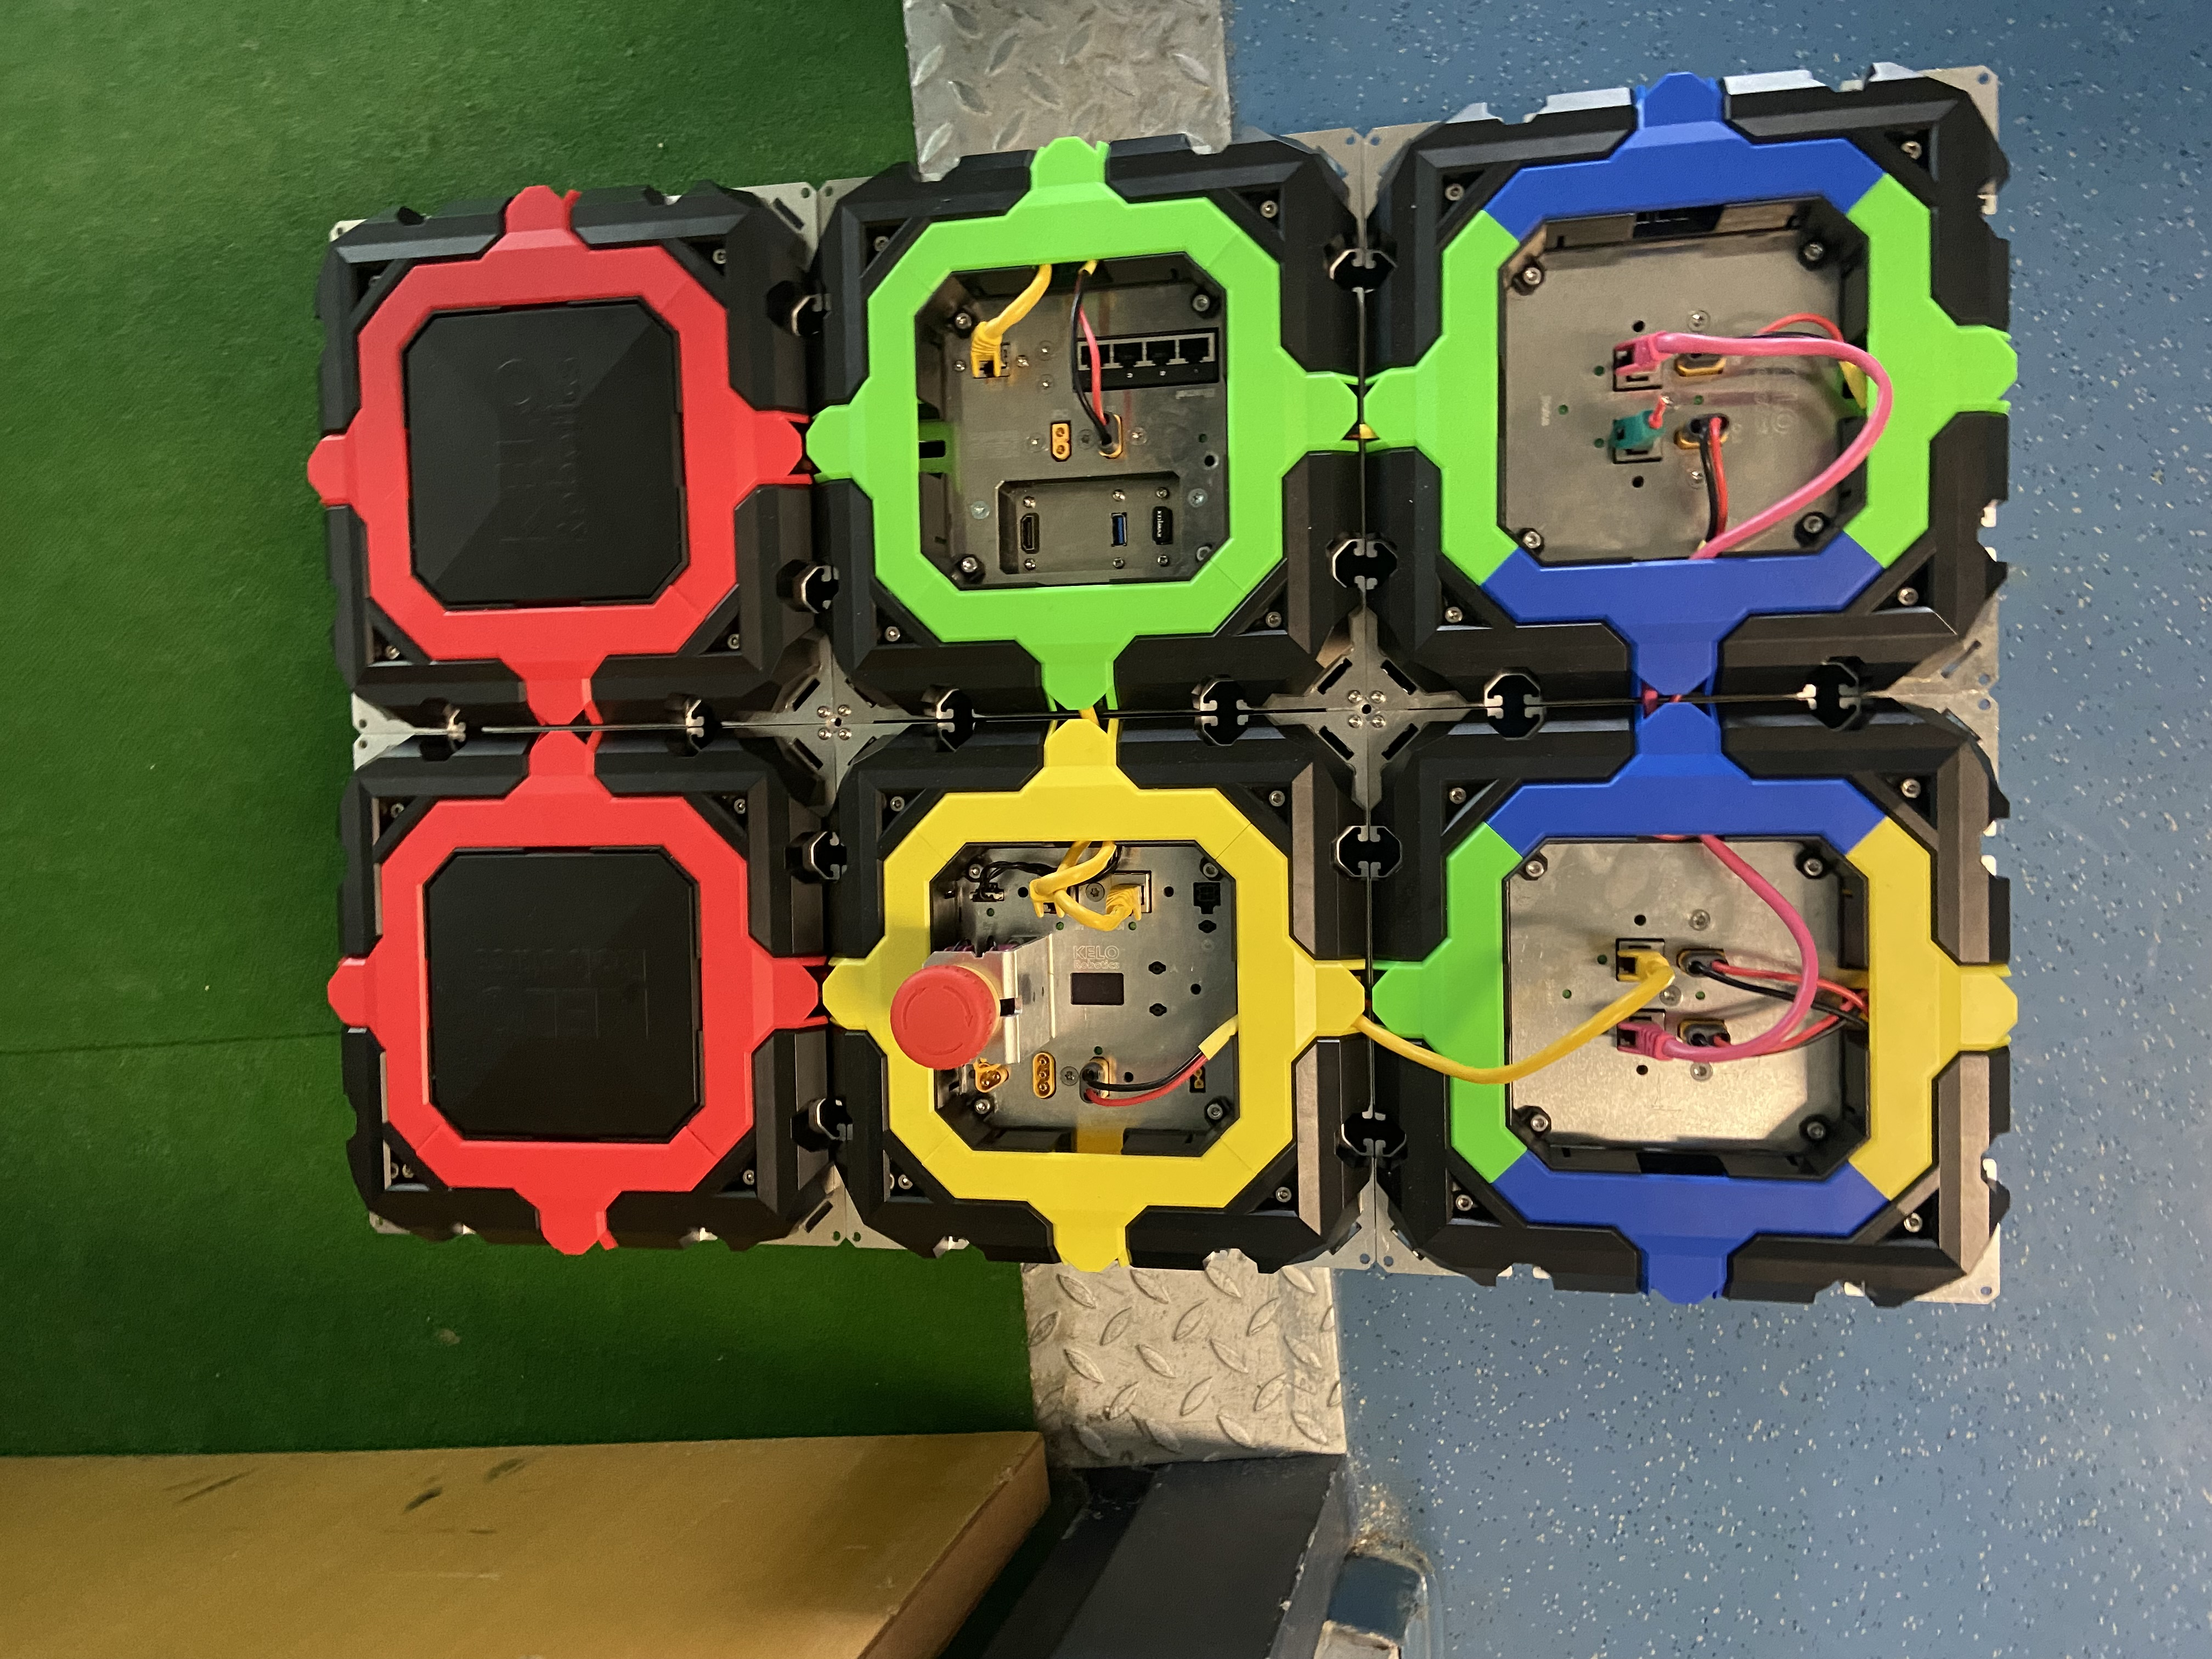
\includegraphics[width=5cm\textwidth, height= 4cm, angle=270, origin=c]{top_view.jpg}}
            \hspace{2em}
            \subfloat[Rear view]{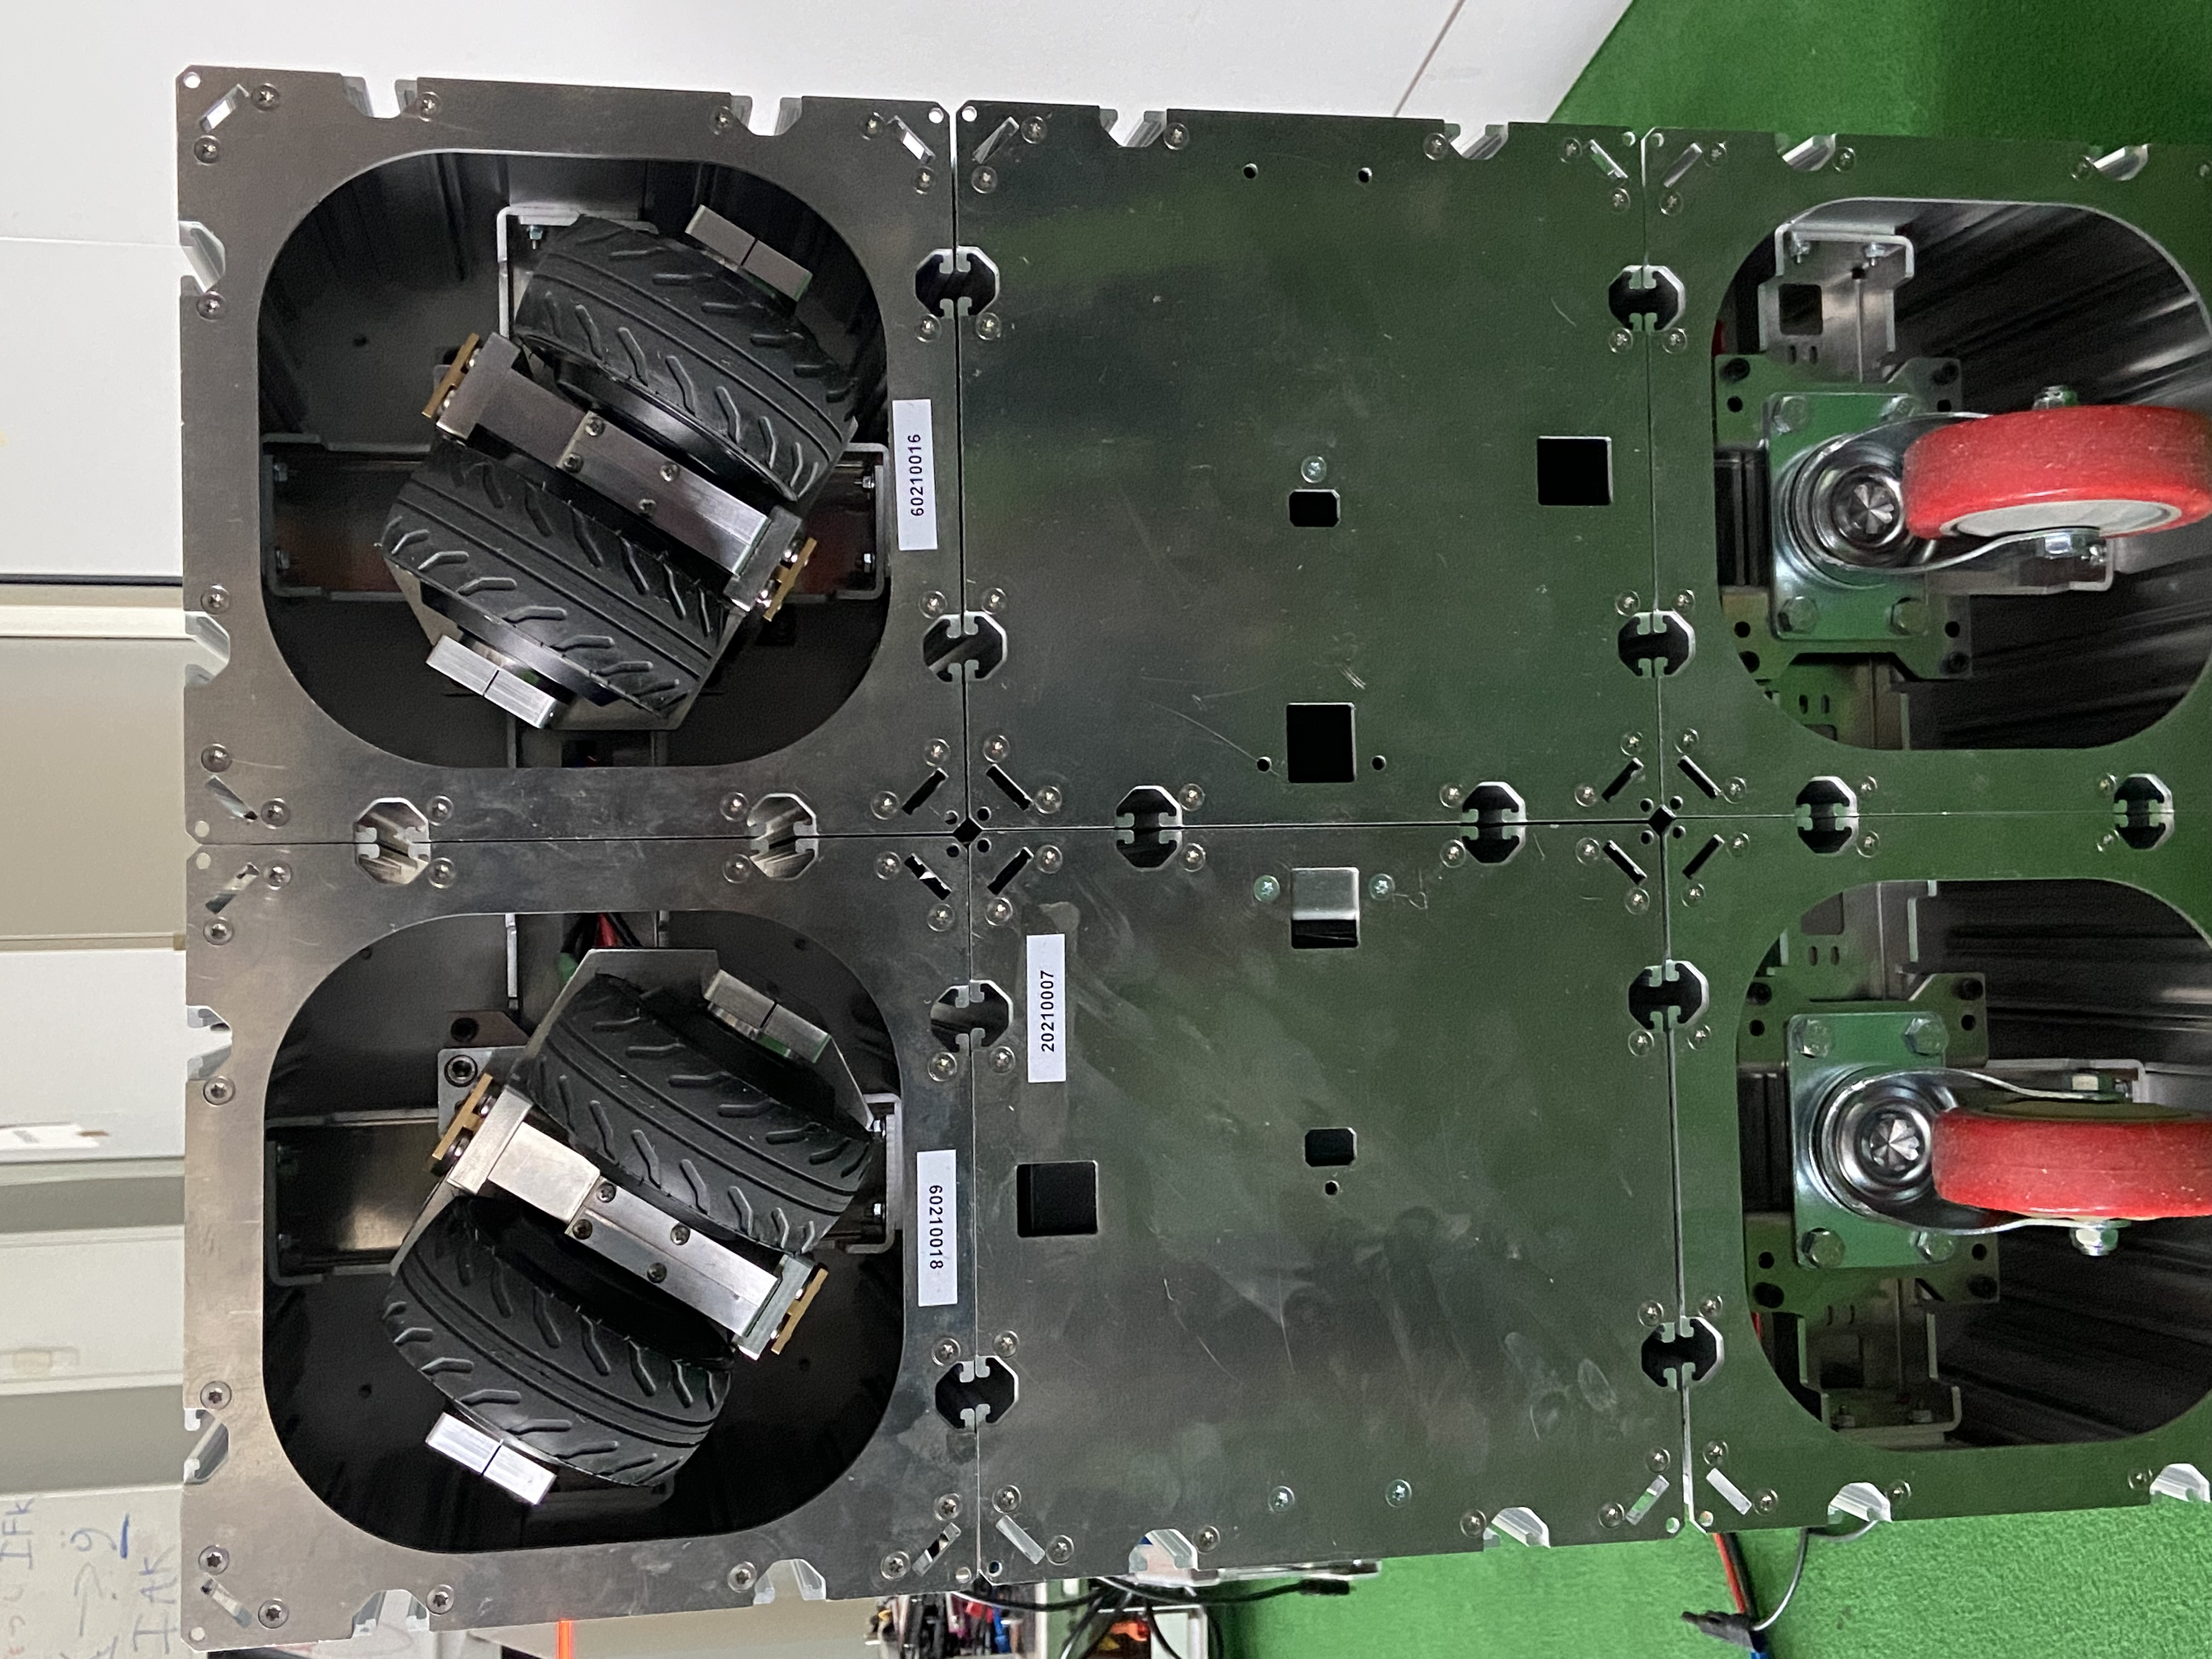
\includegraphics[width=5cm\textwidth , height= 4cm, angle=270, origin=c]{4_wheel_config.jpg}} \\[0.25cm]
            \caption{Top and rear view of Robot Freddy }
            \label{fig:wheels}
        \end{figure}
\end{frame}
\begin{frame}{Problem definition}
\begin{tcolorbox}[colback=blue!5!white,colframe=blue!75!black]
Safe ramping behaviour of Freddy robot using motion primitives.
\end{tcolorbox}

      \begin{tikzpicture}[overlay,remember picture]
        \node[anchor=south east,xshift=-30pt,yshift=35pt]
          at (current page.south east) {
            %\includegraphics[width=35mm]{resources/jabberwocky-light}
          };
      \end{tikzpicture}%
\end{frame}

\begin{frame}{Velocity control - video}


      \begin{tikzpicture}[overlay,remember picture]
        \node[anchor=south east,xshift=-30pt,yshift=35pt]
          at (current page.south east) {
            %\includegraphics[width=35mm]{resources/jabberwocky-light}
          };
      \end{tikzpicture}%
      \begin{figure}[H]
            \centering
            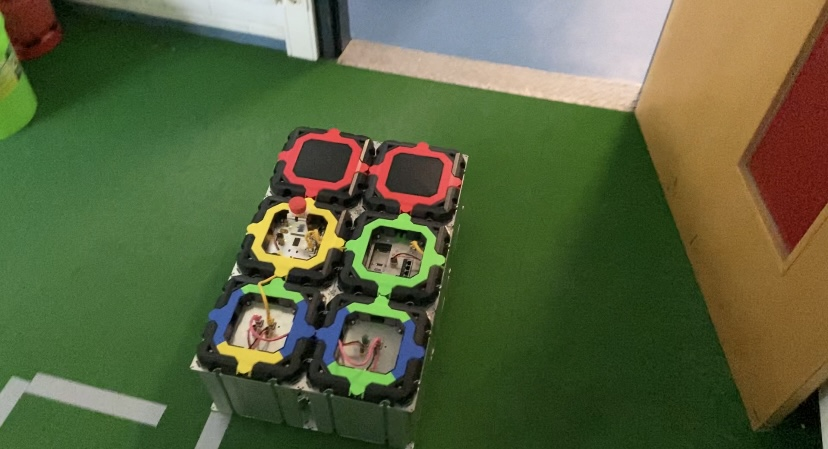
\includegraphics[width= 8cm, height= 5.5cm]{velocity_control.jpg}
        \end{figure}
\end{frame}

\begin{frame}{Safe ramping behaviour - video}

      \begin{tikzpicture}[overlay,remember picture]
        \node[anchor=south east,xshift=-30pt,yshift=35pt]
          at (current page.south east) {
            %\includegraphics[width=35mm]{resources/jabberwocky-light}
          };
      \end{tikzpicture}%
      
      \begin{figure}[H]
            \centering
            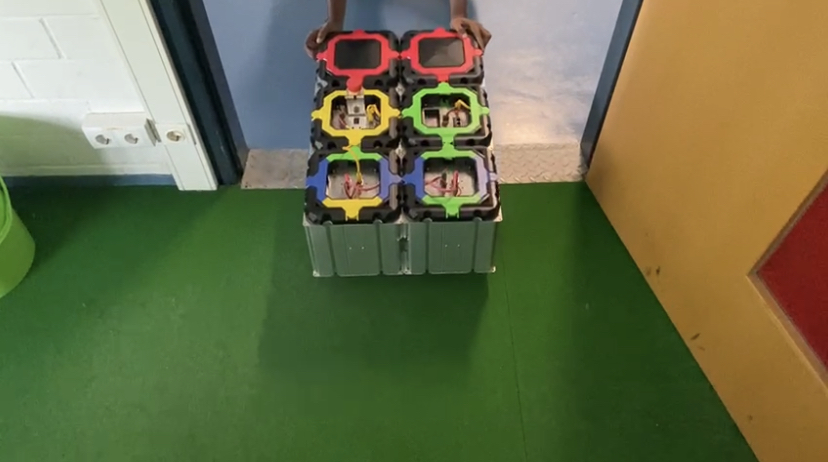
\includegraphics[width= 8cm, height= 5.5cm]{Safe_ramping_beh.jpg}
        \end{figure}
\end{frame}

\begin{frame}{Push/pull configuration - video}


      \begin{tikzpicture}[overlay,remember picture]
        \node[anchor=south east,xshift=-30pt,yshift=35pt]
          at (current page.south east) {
            %\includegraphics[width=35mm]{resources/jabberwocky-light}
          };
      \end{tikzpicture}%
      \begin{figure}[H]
            \centering
            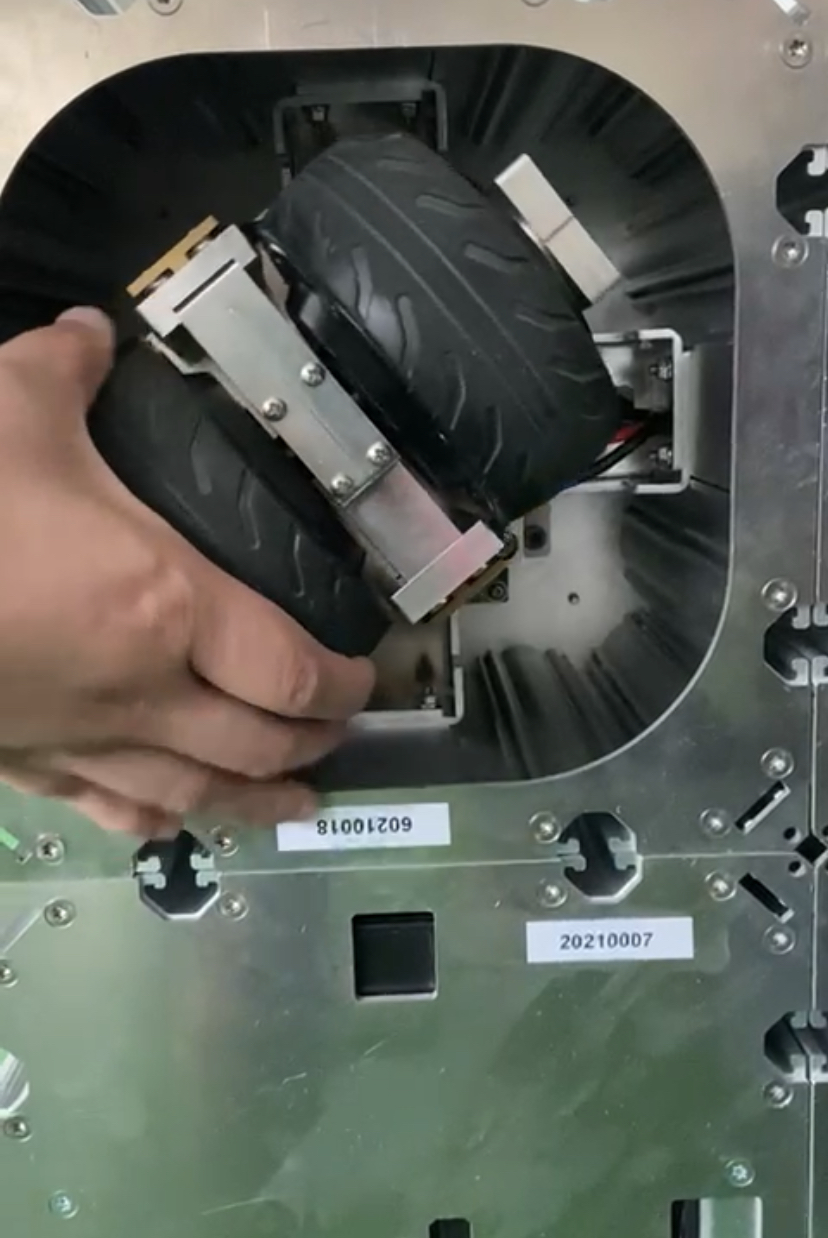
\includegraphics[width= 5cm, height= 6cm]{push_pull.jpg}
        \end{figure}
\end{frame}
\begin{frame}{Wheel configuration}


      \begin{tikzpicture}[overlay,remember picture]
        \node[anchor=south east,xshift=-30pt,yshift=35pt]
          at (current page.south east) {
            %\includegraphics[width=35mm]{resources/jabberwocky-light}
          };
      \end{tikzpicture}%
      \begin{figure}[H]
            \centering
            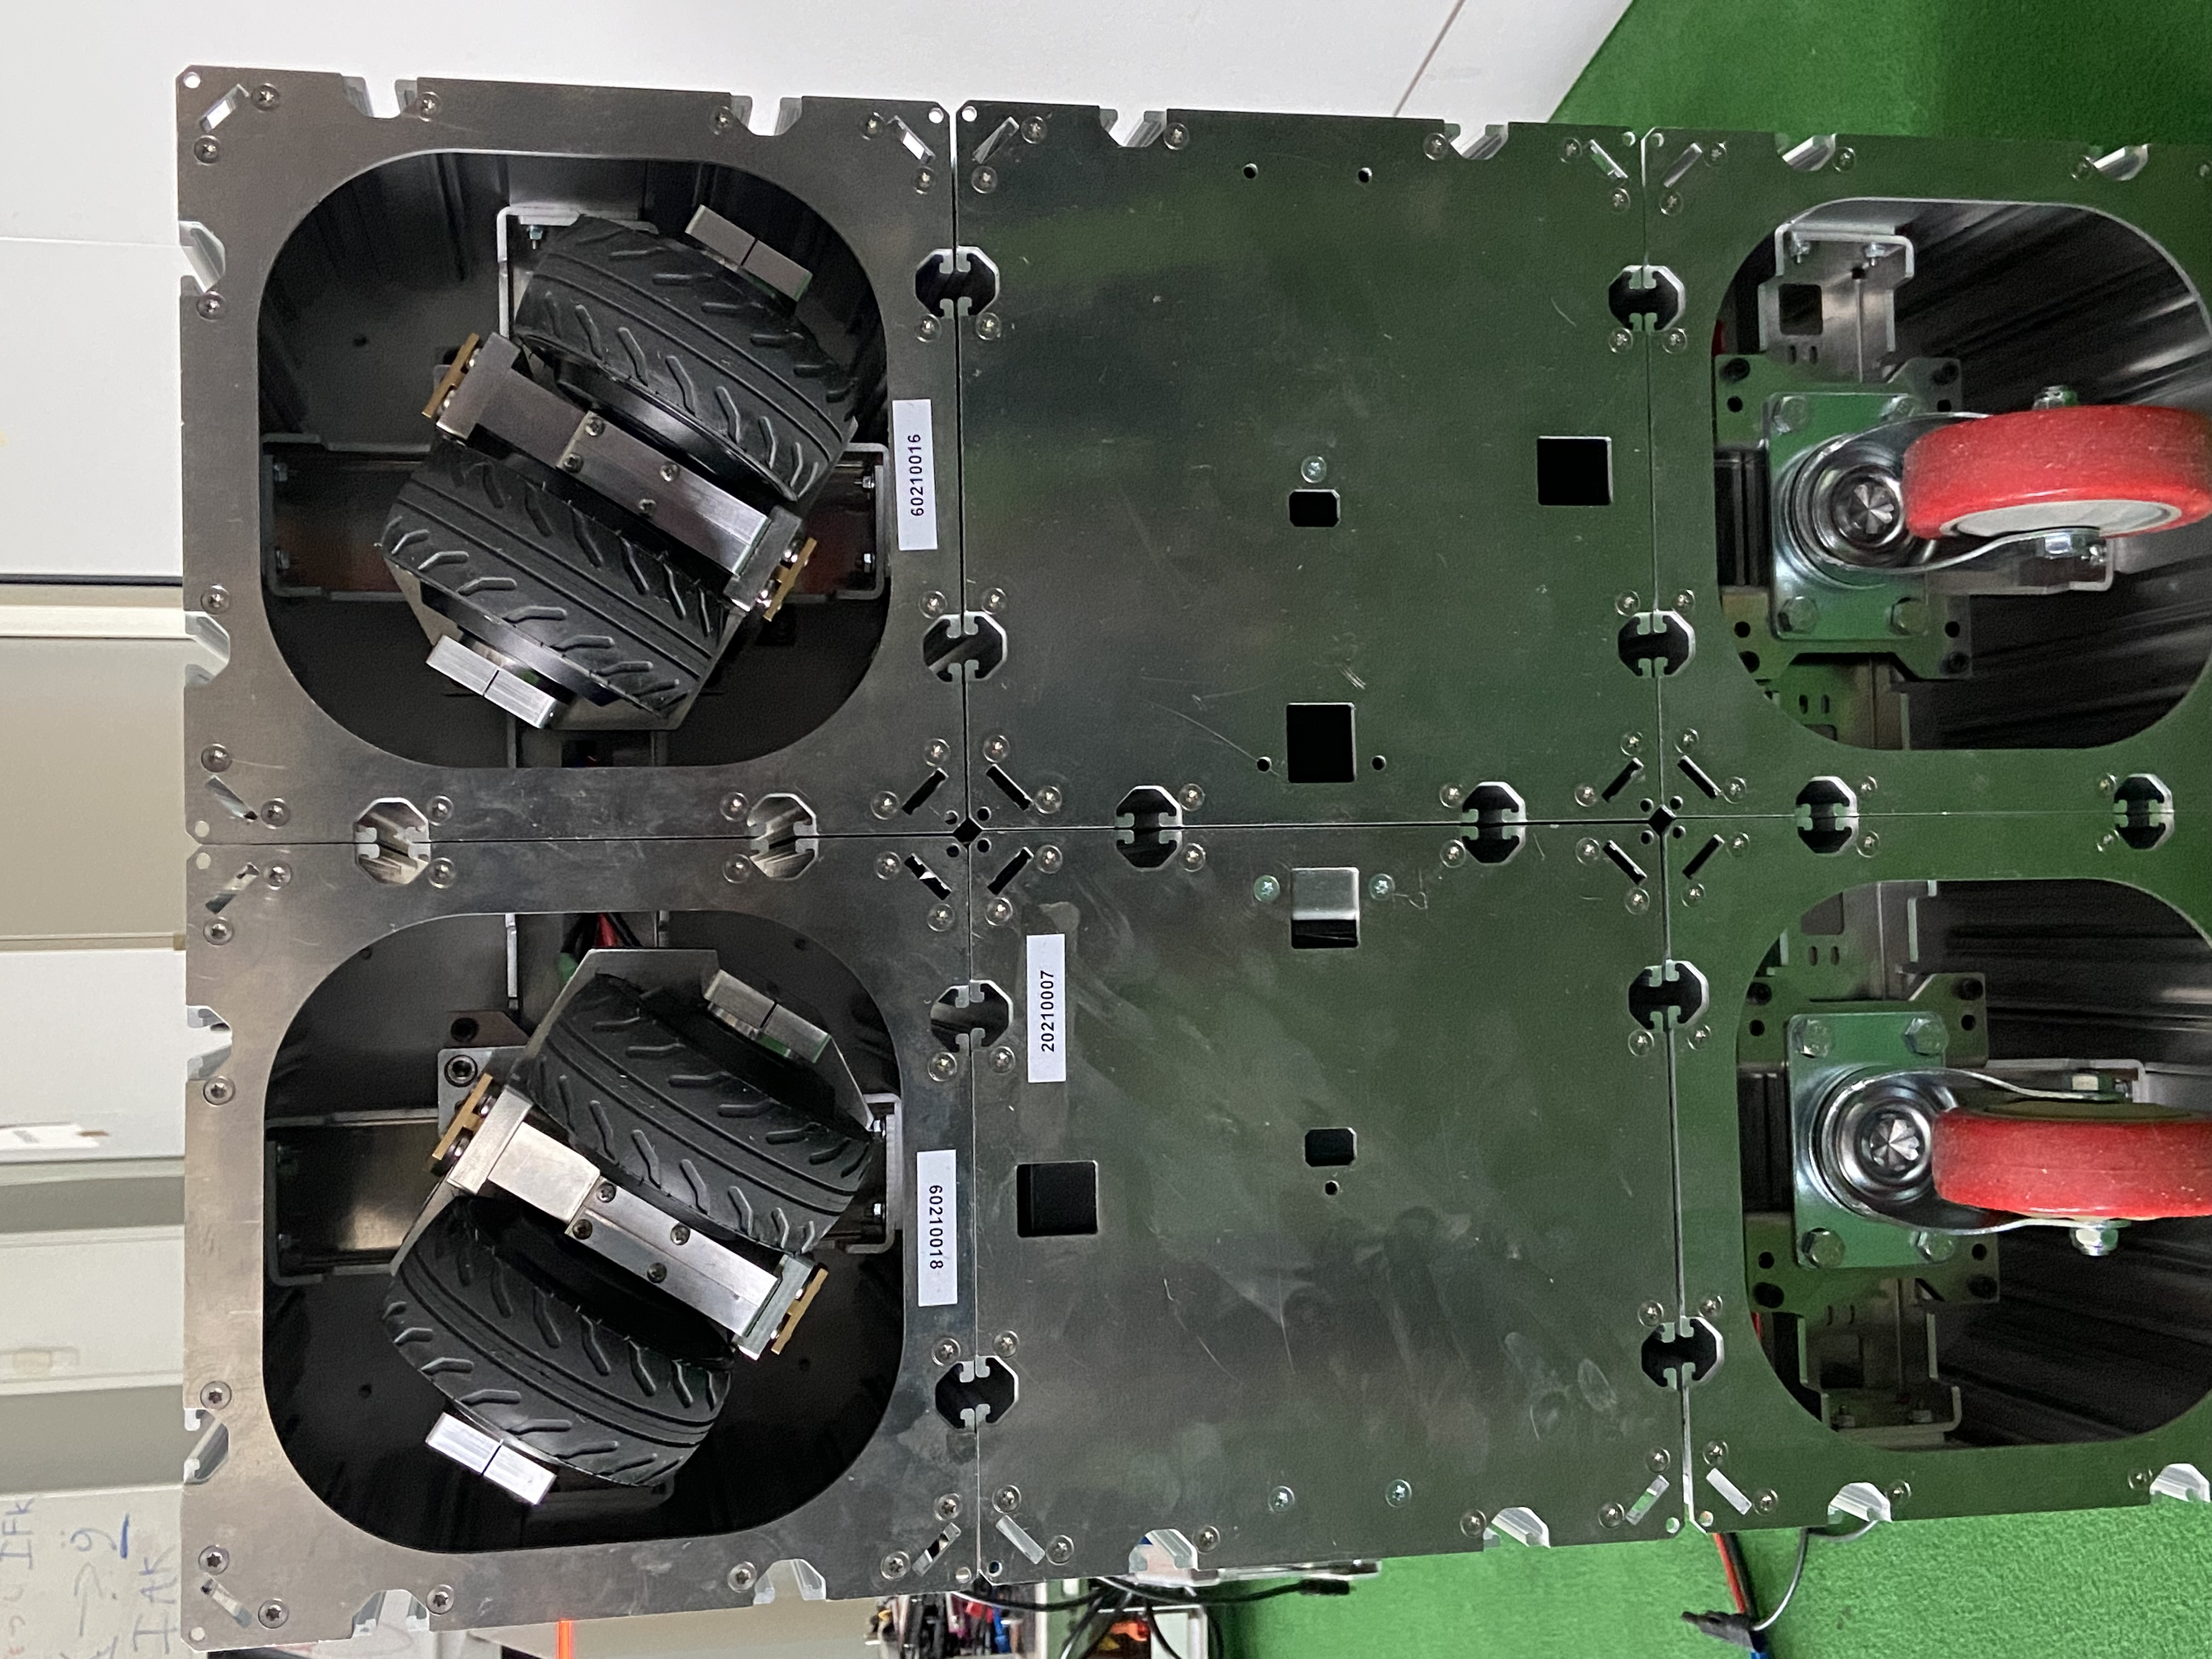
\includegraphics[width= 6.5cm, height= 5cm,angle=270,origin=c]{4_wheel_config.jpg}
        \end{figure}
\end{frame}

\begin{frame}{Top view of 2 castor and 2 active wheels configuration}

      \begin{tikzpicture}[overlay,remember picture]
        \node[anchor=south east,xshift=-30pt,yshift=35pt]
          at (current page.south east) {
            %\includegraphics[width=35mm]{resources/jabberwocky-light}
          };
      \end{tikzpicture}%
      \begin{figure}[H]
            \centering
            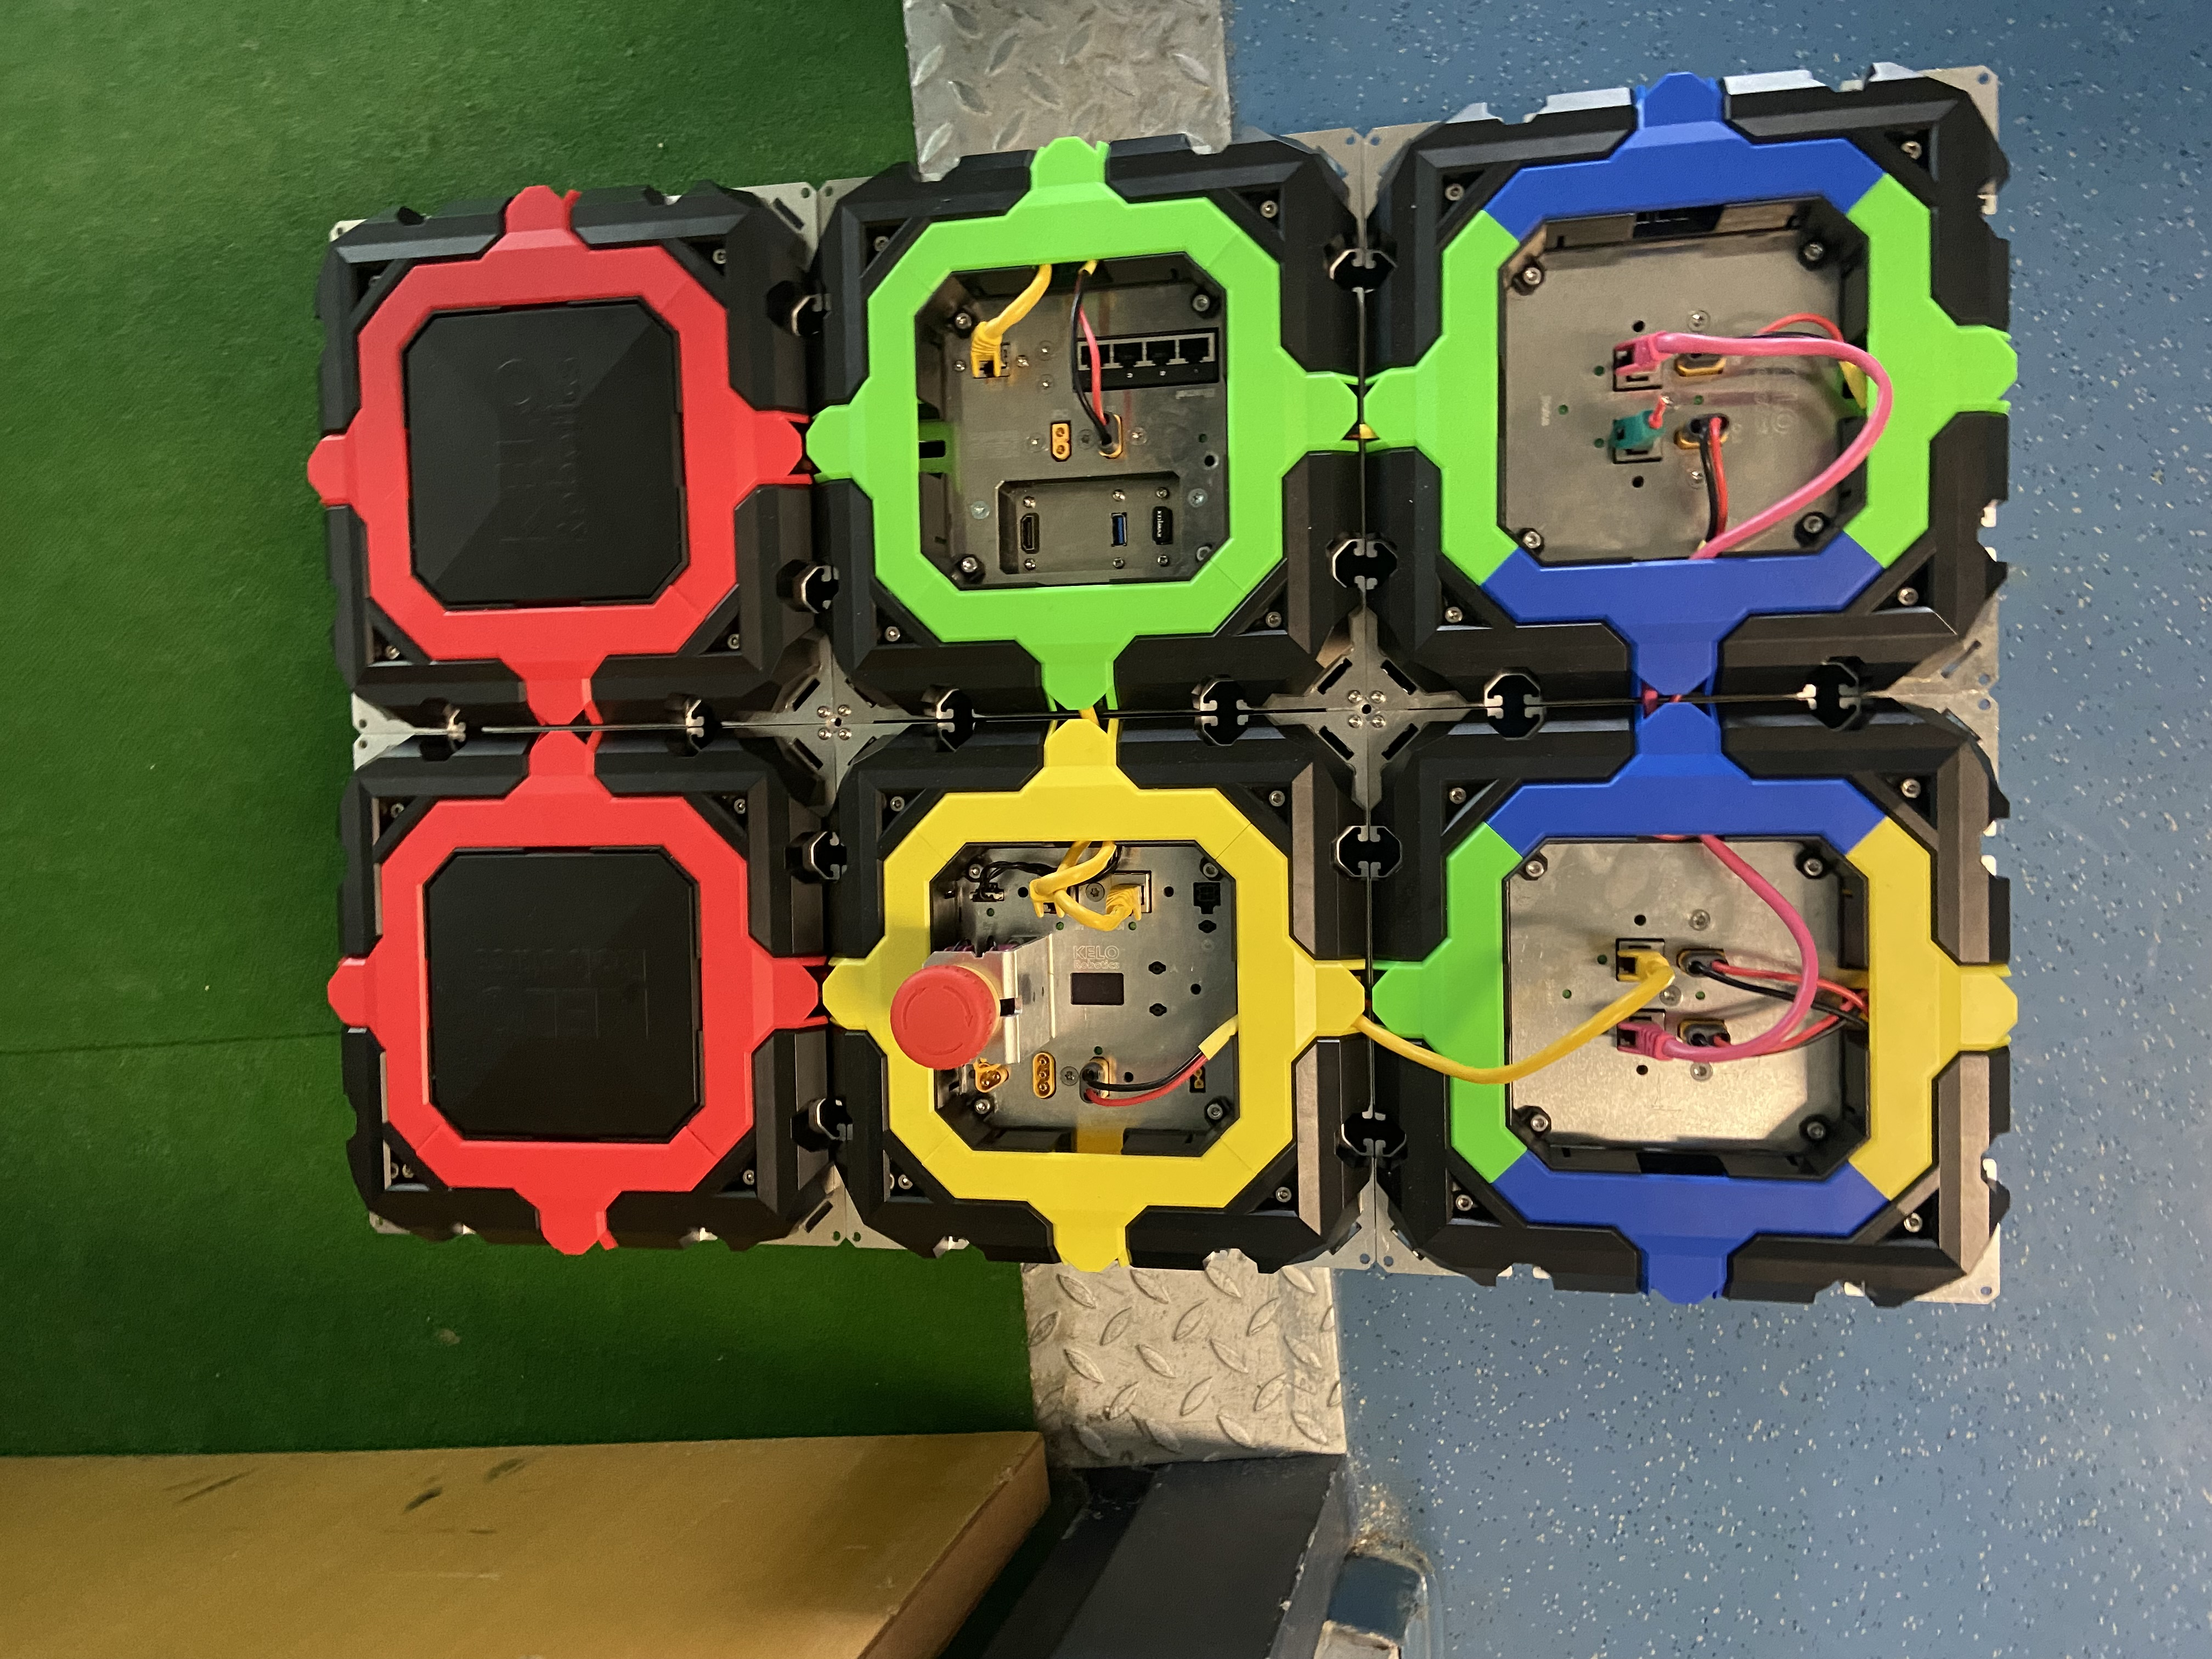
\includegraphics[width= 6cm, height= 5cm,angle=270,origin=c]{top_view.jpg}
        \end{figure}
\end{frame}

\begin{frame}{Project goal}
\begin{tcolorbox}[colback=blue!5!white,colframe=blue!75!black]
Successfully perform the ramping motion on the Freddy robot safely.
\end{tcolorbox}

      \begin{tikzpicture}[overlay,remember picture]
        \node[anchor=south east,xshift=-30pt,yshift=35pt]
          at (current page.south east) {
            %\includegraphics[width=35mm]{resources/jabberwocky-light}
          };
      \end{tikzpicture}%
\end{frame}


\begin{frame}{Required libraries}
\begin{itemize}
    \item Simple Open EtherCAT Master (SOEM) - communication between robot and the actuators. \footnote{\href{https://github.com/OpenEtherCATsociety/SOEM}{SOEM github repository}}
    \item robif2b - robot control interface \footnote{\href{https://github.com/rosym-project/robif2b}{robif2b github repository}}

\end{itemize}


      \begin{tikzpicture}[overlay,remember picture]
        \node[anchor=south east,xshift=-30pt,yshift=35pt]
          at (current page.south east) {
            %\includegraphics[width=35mm]{resources/jabberwocky-light}
          };
      \end{tikzpicture}%
\end{frame}


\begin{frame}{User story 1}
 \begin{figure}[H]
            \centering
            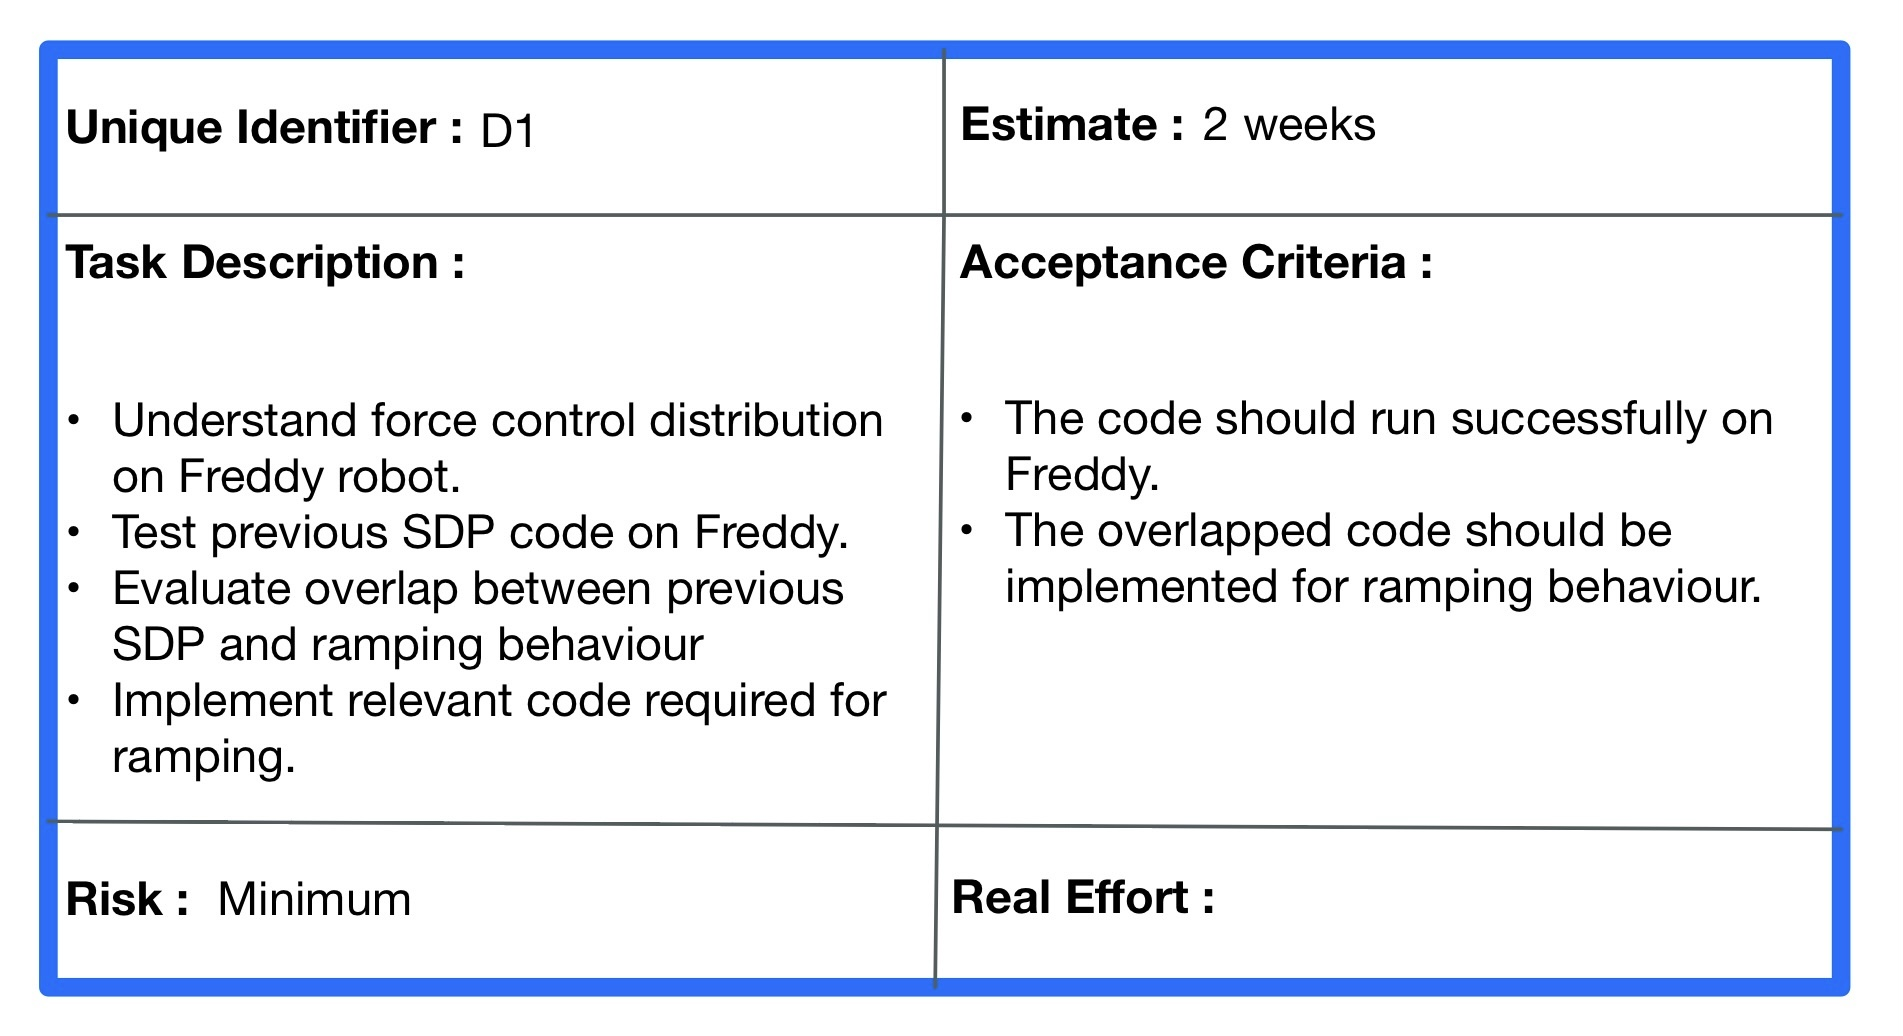
\includegraphics[width=11cm  , height= 6cm]{user_story1.jpg}
        \end{figure}
      \begin{tikzpicture}[overlay,remember picture]
        \node[anchor=south east,xshift=-30pt,yshift=35pt]
          at (current page.south east) {
            %\includegraphics[width=35mm]{resources/jabberwocky-light}
          };
      \end{tikzpicture}%
\end{frame}


\begin{frame}{User story 2}
\begin{figure}[H]
            \centering
            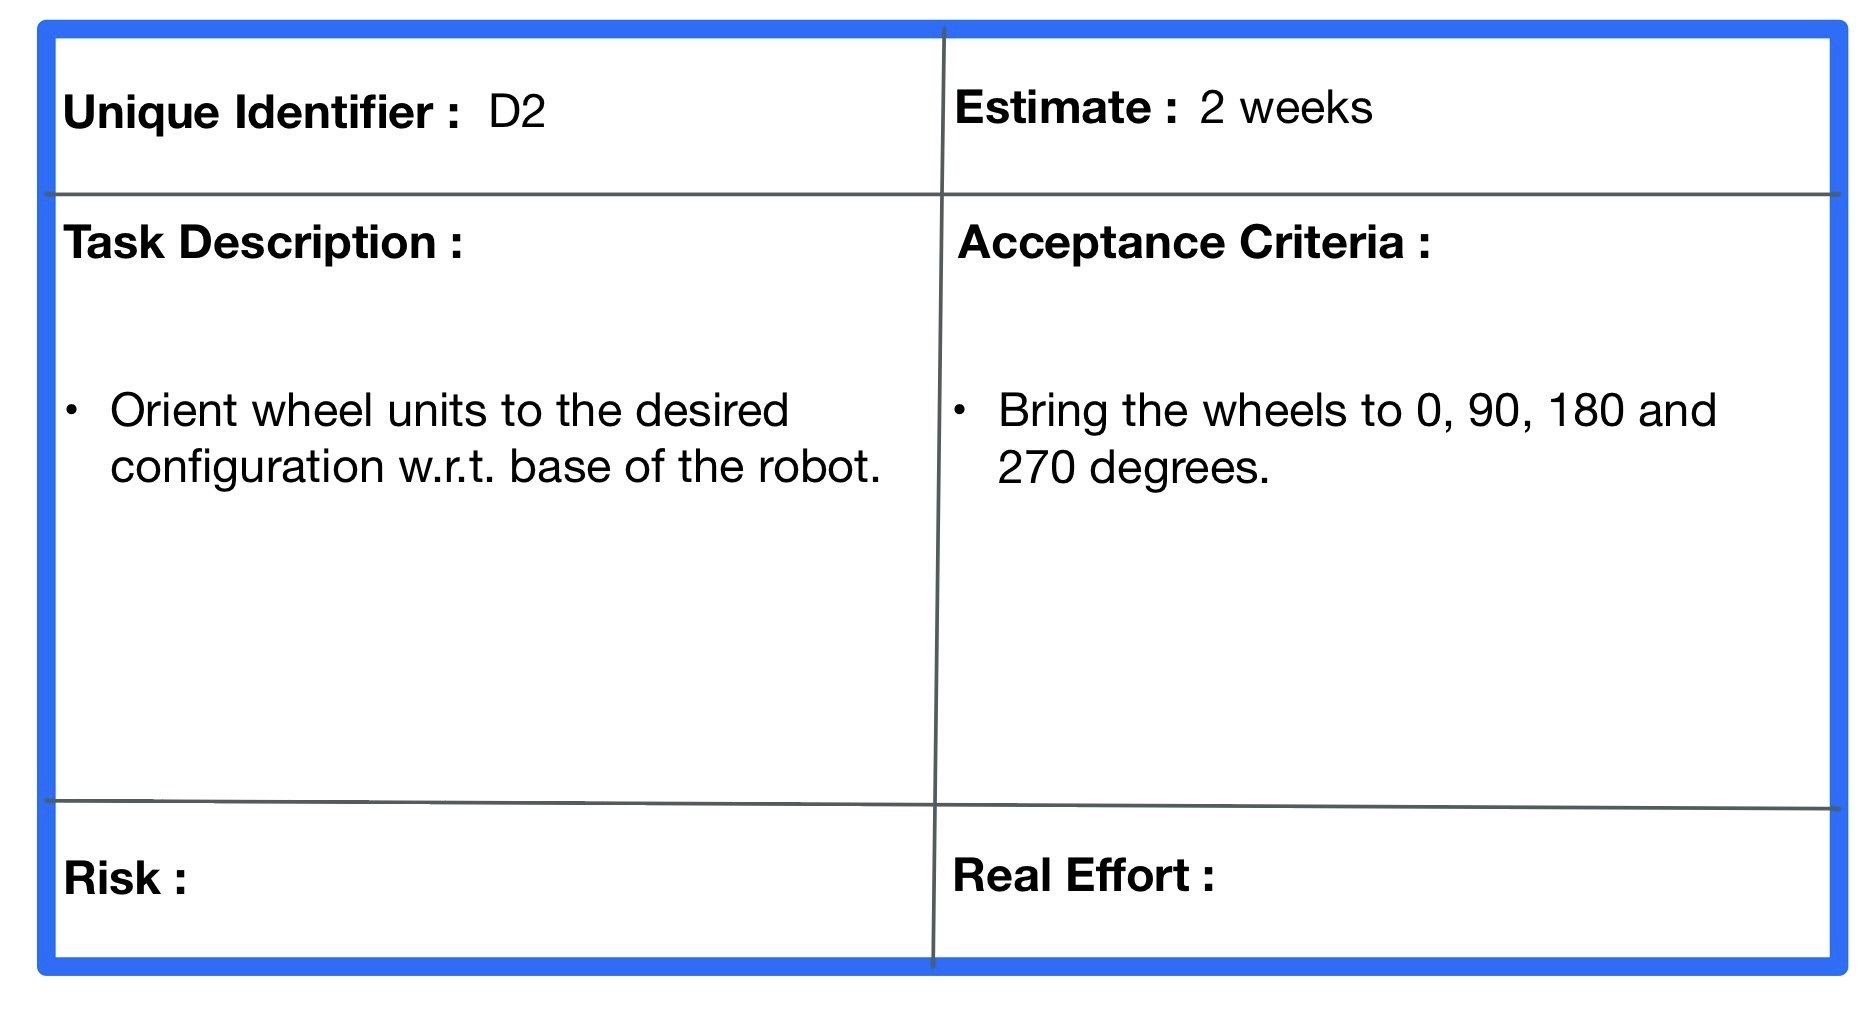
\includegraphics[width=11cm  , height= 6cm]{user_story2.jpg}
        \end{figure}

      \begin{tikzpicture}[overlay,remember picture]
        \node[anchor=south east,xshift=-30pt,yshift=35pt]
          at (current page.south east) {
            %\includegraphics[width=35mm]{resources/jabberwocky-light}
          };
      \end{tikzpicture}%
\end{frame}


\begin{frame}{User story 3}
\begin{figure}[H]
            \centering
            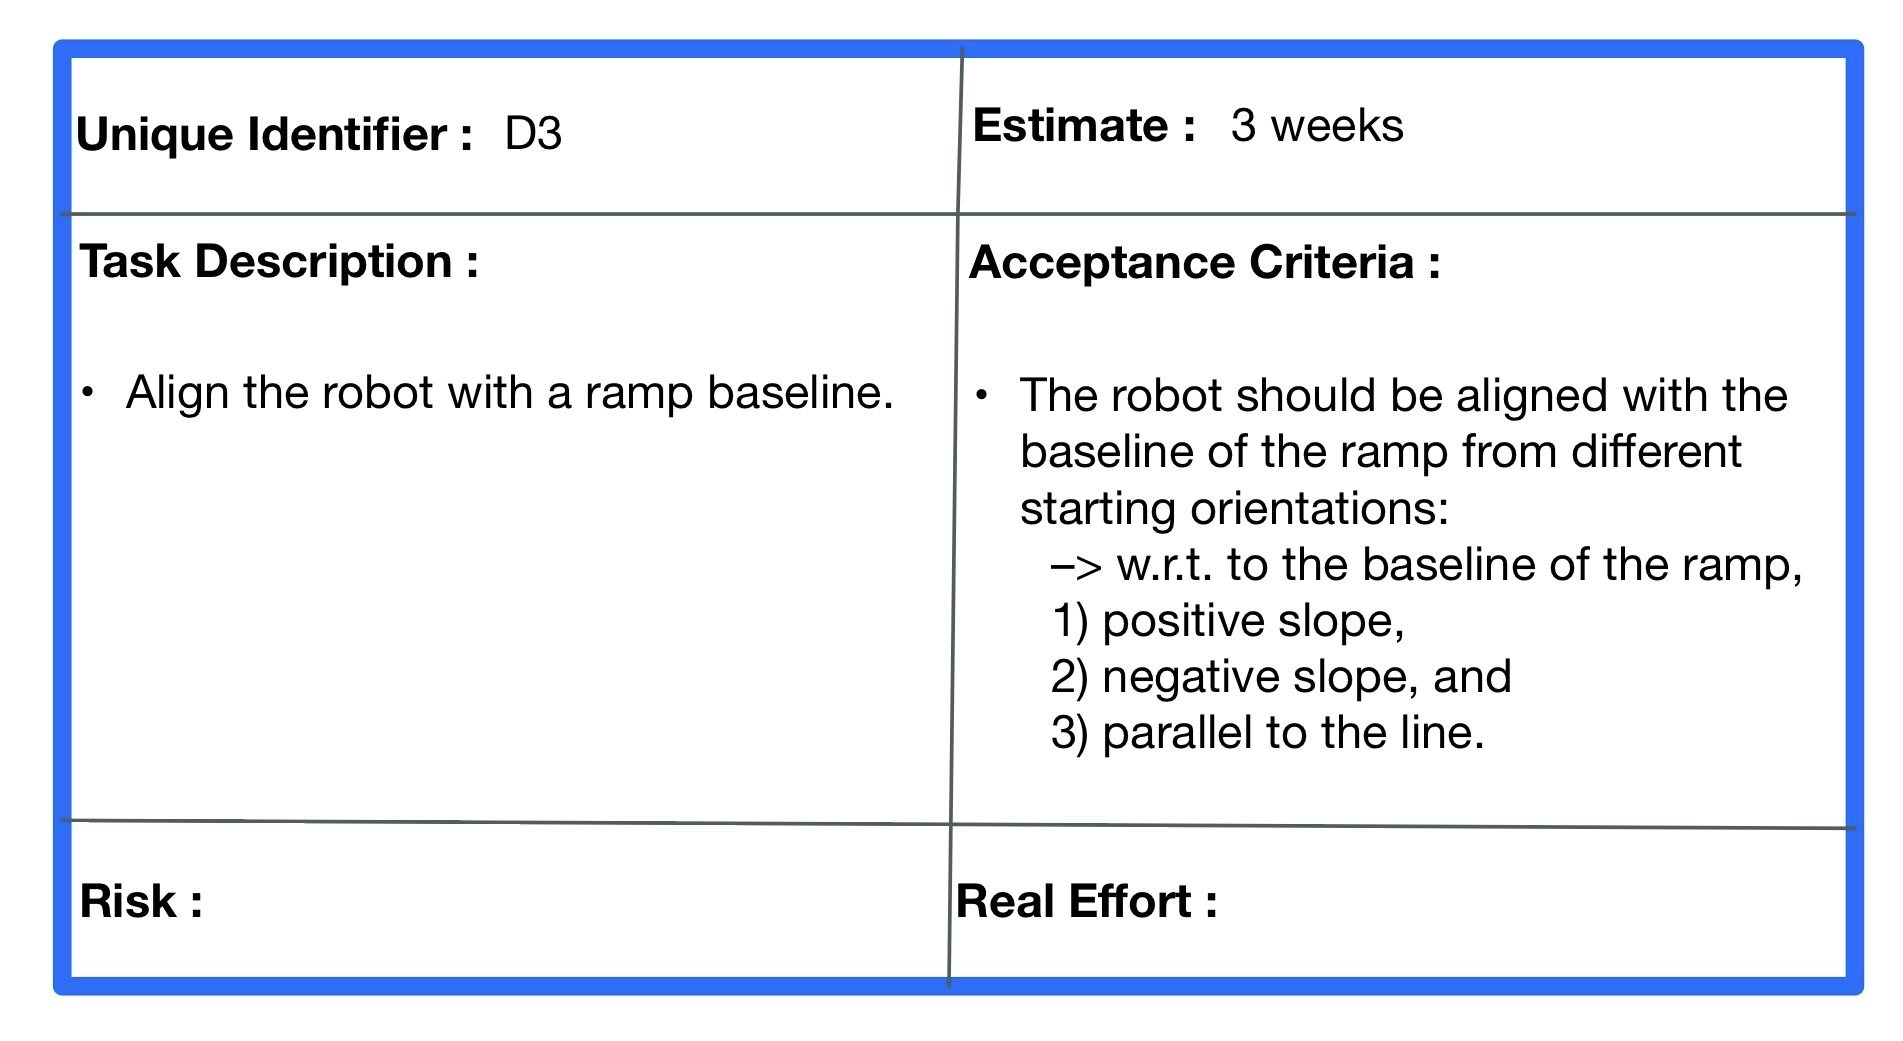
\includegraphics[width=11cm  , height= 6cm]{user_story3.jpg}
        \end{figure}
      \begin{tikzpicture}[overlay,remember picture]
        \node[anchor=south east,xshift=-30pt,yshift=35pt]
          at (current page.south east) {
            %\includegraphics[width=35mm]{resources/jabberwocky-light}
          };
      \end{tikzpicture}%
\end{frame}

\begin{frame}{Robot alignment w.r.t. ramp}
\begin{figure}[H]
            \centering
            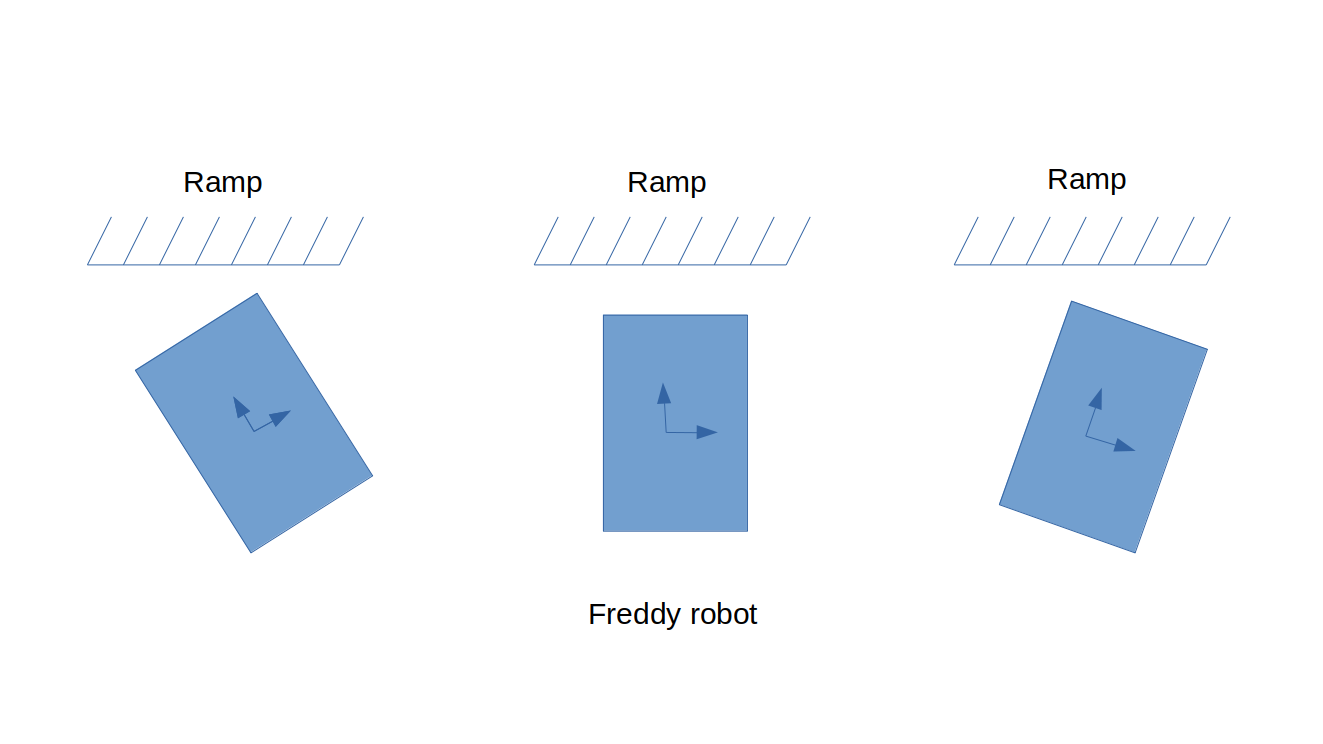
\includegraphics[width=11cm  , height= 6cm]{freddy_robot_alignment.png}
        \end{figure}
      \begin{tikzpicture}[overlay,remember picture]
        \node[anchor=south east,xshift=-20pt,yshift=35pt]
          at (current page.south east) {
            %\includegraphics[width=35mm]{resources/jabberwocky-light}
          };
      \end{tikzpicture}%
\end{frame}

\begin{frame}{User story 4}
\begin{figure}[H]
            \centering
            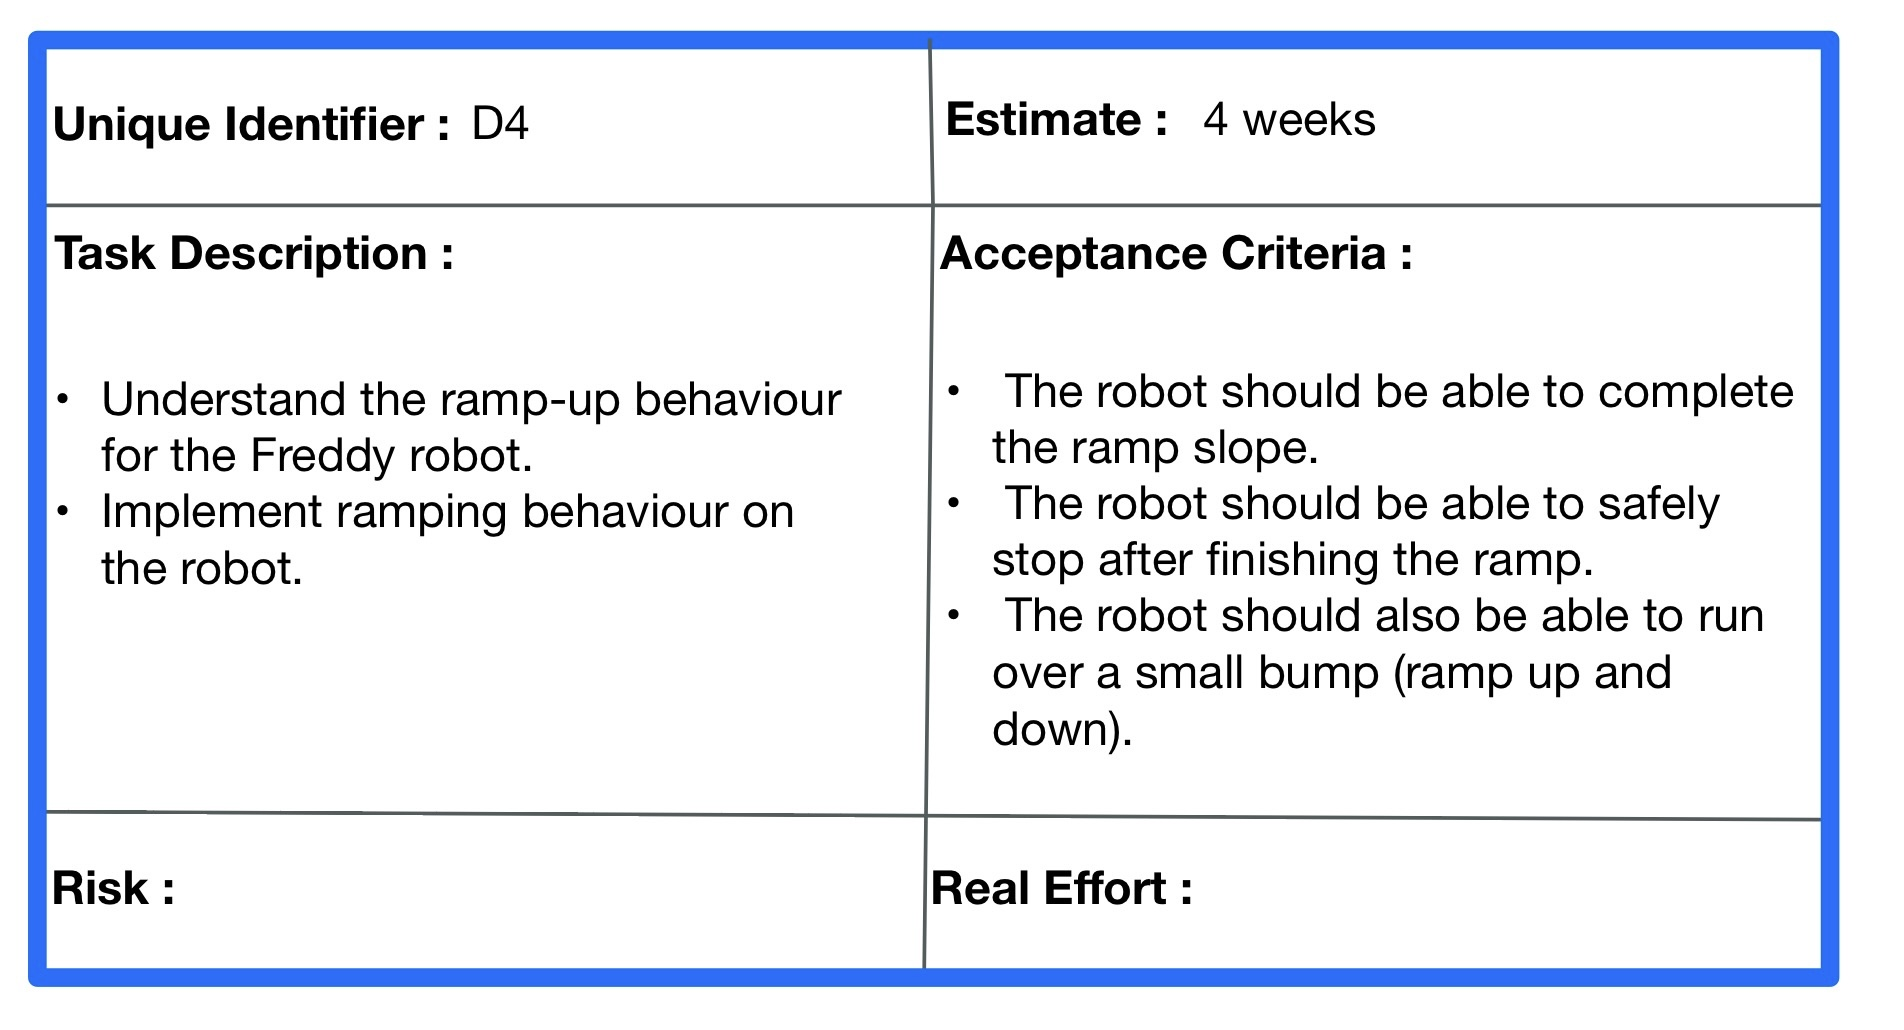
\includegraphics[width=11cm  , height= 6cm]{user_story4.jpg}
        \end{figure}
      \begin{tikzpicture}[overlay,remember picture]
        \node[anchor=south east,xshift=-30pt,yshift=35pt]
          at (current page.south east) {
            %\includegraphics[width=35mm]{resources/jabberwocky-light}
          };
      \end{tikzpicture}%
\end{frame}


\begin{frame}{User story 5}
\begin{figure}[H]
            \centering
            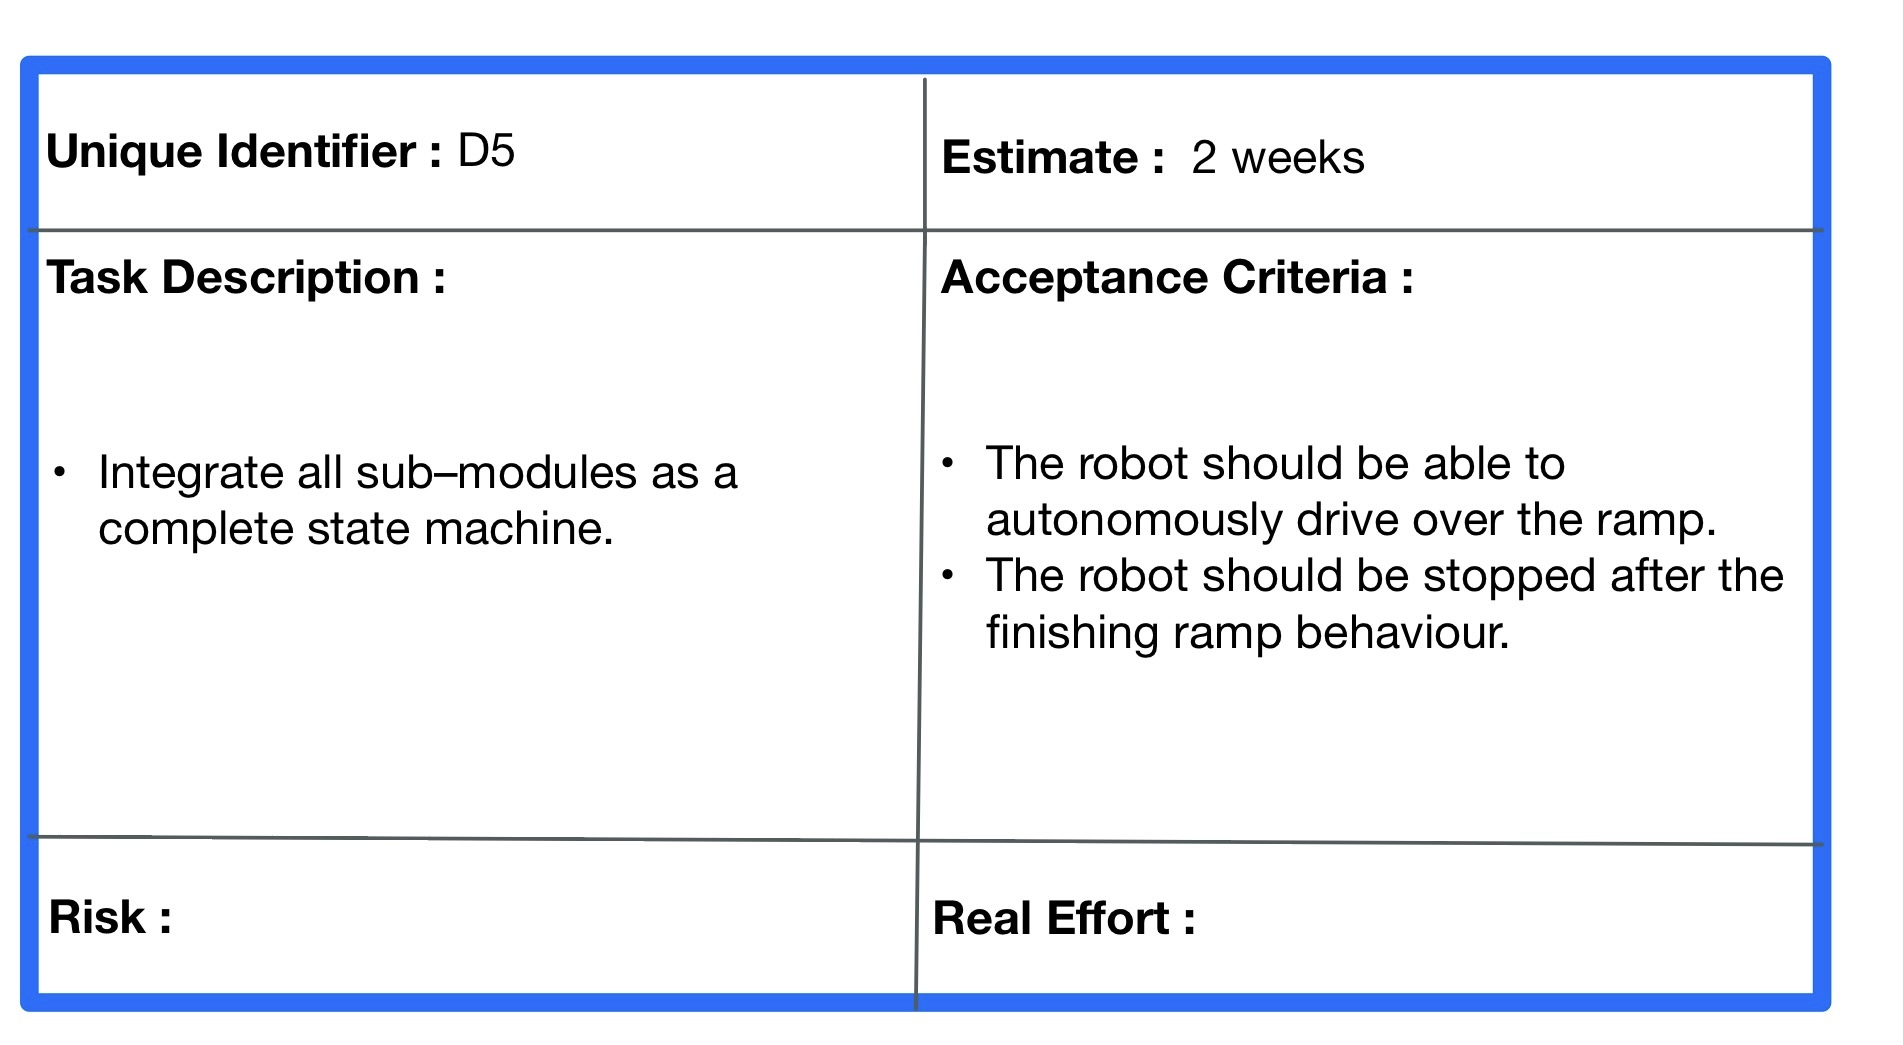
\includegraphics[width=11cm  , height= 6cm]{user_story5.jpg}
        \end{figure}

      \begin{tikzpicture}[overlay,remember picture]
        \node[anchor=south east,xshift=-30pt,yshift=35pt]
          at (current page.south east) {
            %\includegraphics[width=35mm]{resources/jabberwocky-light}
          };
      \end{tikzpicture}%
\end{frame}


\begin{frame}{Collaboration plans}
\begin{figure}[H]
            \centering
            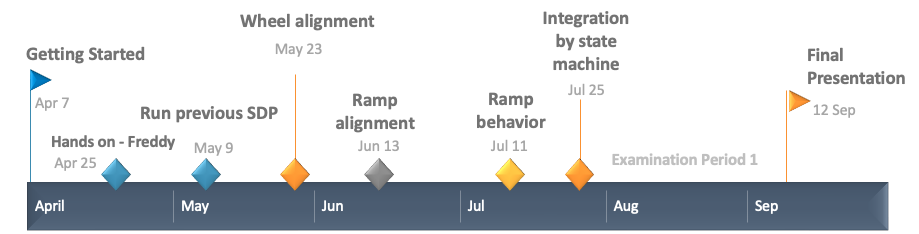
\includegraphics[width=11cm  , height= 3cm]{roadmap.png}
            \caption{Project Roadmap}
            \label{fig:roadmap}
        \end{figure}
Version Control : GIT: \href{https://github.com/HBRS-SDP/ss22-motion-primitive-freddy}{Motion Primitive Freddy repository} 

Communication medium: Slack

Meeting frequency :  Internal meeting twice a week and with the Advisor, every Monday (in-person/online)

\end{frame}

\end{document}
